\documentclass[a4paper,10pt, oneside]{article}
\usepackage[utf8]{inputenc}
\usepackage[T1]{fontenc}
\usepackage[spanish]{babel}
\usepackage[style=ieee,backend=bibtex]{biblatex}
\usepackage{graphicx}
\usepackage{amsmath}
\usepackage{pgfplots}
\usepackage{lineno}
%\usepackage{showframe}
\usepackage[top=1in, bottom=1.25in, left=1.25in, right=1.25in]{geometry}
\usepackage{caption}
\usepackage{bytefield}
\usepackage{amsmath}
\usepackage{csquotes}
\usepackage{svg}
\usepackage{lscape}
\usepackage{multicol}
\usepackage{subfig}
\usepackage{hyperref}
\usepackage{pgfplots, pgfplotstable}




\usepackage{listings,xcolor}
\lstset{
	string=[s]{"}{"},
	stringstyle=\color{blue},
	comment=[l]{:},
	commentstyle=\color{black},
}


\bibliography{informe_3}

	
\begin{document}
	
\begin{titlepage}
	\centering
	
\includegraphics[width=0.25\textwidth]{../../Universidad_del_Litoral}\par\vspace{1cm}
	{\scshape\LARGE Universidad Nacional del Litoral \par}
	\vspace{1cm}
	{\scshape\Large Proyecto Final de Carrera\par}
	\vspace{1.5cm}
	{\huge\bfseries Diseño de un sistema de detección de anomalías en redes de computadoras.\par}
	\vspace{4cm}
	{\huge\bfseries Informe de avance 3\par}
	\vfill
	
	{\Large \itshape Pineda Leandro\par}
	
	
	% Bottom of the page
	\large Córdoba\par
	{\large \today\par}	
\end{titlepage}

\modulolinenumbers[5]
\linenumbers

\section{Introducción}


\section{Comunicación entre componentes}
La arquitectura de un sistema es la descripción de su estructura en términos de componentes específicos y sus interrelaciones. Mediante esta modularización, podemos asegurarnos que dicha estructura satisface las demandas actuales (es decir, resuelve el problema para el cual fue construido) y puede ser adaptada para satisfacer demandas futuras.
Podemos definir a los sistemas distribuidos como aquellos compuestos por varios componentes que no comparten el mismo espacio de memoria\cite{Muhl:2006:DES:1162246}. Cuando se diseñan sistemas distribuidos es necesario considerar lo siguiente: 

\begin{itemize}
	\item ¿Cuales son las entidades que se comunican entre si?
	\item ¿Cómo van a comunicarse, o para ser mas específicos, que paradigma de comunicación va a usarse?
\end{itemize}

Estas preguntas son centrales para entender los sistemas distribuidos; qué se está comunicando y cómo esas entidades se comunican entre si, definen una gran cantidad de variables a ser consideradas por quienes construyen estos sistemas.

Las entidades que se comunican en un sistema distribuido son típicamente procesos, lo que nos permite entender a los sistemas distribuidos como procesos que se relacionan mediante los paradigmas de comunicación \textit{entre procesos} apropiados. Podemos nombrar tres paradigmas de comunicación:

\begin{itemize}
	\item Comunicación \textit{entre procesos}.
	\item Invocación remota.
	\item Comunicación indirecta.
\end{itemize}

\paragraph{Comunicación entre procesos}
La comunicación \textit{entre procesos} refiere al soporte de bajo nivel para la comunicación entre procesos en sistemas distribuidos, incluyendo primitivas para manejo de mensajes, acceso directo a las API provistas por protocolos de Internet (esto es, usando Sockets) y soporte para comunicación \textit{multicast}.

Para comunicarse, un proceso envía un mensaje (una secuencia de bytes) a un receptor y un procesos ejecutandose allí recibe el mensaje. Esta actividad involucra el pasaje de datos de un proceso emisor a un proceso receptor y puede significar la sincronización de ambos procesos.

\paragraph{Invocación remota}
La invocación remota representa el paradigma de comunicación más común en sistemas distribuidos. El intercambio de mensajes entre las entidades comunicantes es bidireccional, de forma que operaciones remotas, procedimientos y métodos, pueden ser invocados como se define a continuación:
\begin{itemize}
	\item Protocolos \textit{request-reply}: estos protocolos involucran el intercambio de mensajes desde el cliente al servidor y luego del servidor al cliente, donde el primer mensaje representa la operación que será ejecutada en el servidor (con los parámetros necesarios) y el segundo contiene cualquier resultado de dicha operación. Este paradigma es mas bien primitivo, y es utilizado generalmente en sistemas embebidos donde la \textit{performance} es de suma importancia.
	\item \textit{Remote procedure calls} (RPC) o llamadas a procedimientos remotos: este concepto, atribuido inicialmente a Birrel and Nelson [1984], representó un gran cambio en los paradigmas de computación distribuida. En RPC, los procedimientos de los procesos ejecutandose en computadoras remotas pueden ser invocados como si se encontraran el espacio local de memoria. De esta manera, el sistema abstrae aspectos acerca de la distribución, como la codificación de los parámetros y resultados y mecanismo de pasaje mensajes. Este esquema soporta comunicación cliente-servidor pero depende de servidores que ofrezcan un conjunto de operaciones a través de una interfaz de servicio para que los clientes puedan llamar esas operaciones como si estuviesen disponibles localmente.
	\item \textit{Remote method invocation} (RMI) o invocación remota de métodos: RMI es similar a RPC pero utiliza objetos distribuidos. Bajo este paradigma, un objeto cliente puede invocar métodos de un objeto remoto. De la misma forma que con RPC, ciertos detalles de como se implementa la comunicación quedan ocultos al usuario. Algunas implementaciones de RMI pueden incluir, además, soporte para darle a los objetos identidad y la habilidad de usar esos identificadores de objetos en llamadas remotas.
\end{itemize}

\paragraph{Comunicación indirecta}
Las técnicas discutidas hasta aquí tienen una cosa en común: la comunicación representa una relación en ambos sentidos entre el emisor y receptor, con los emisores enviando explícitamente mensajes/invocaciones a los receptores asociados. Los receptores generalmente deben saber sobre la identidad de los emisores y, en la mayoría de los casos, ambas partes deben existir al mismo tiempo para que la comunicación sea exitosa. Lo descrito anteriormente no puede garantizarse en ciertos escenarios. Por esto, surgieron numerosas técnicas donde la comunicación es indirecta a través de una tercera entidad, permitiendo un gran grado de desacople entre emisores y receptores. En particular:
\begin{itemize}
\item Los emisores no necesitan saber a quien le están enviando datos.
\item Emisores y receptores no necesitan existir al mismo tiempo.
\end{itemize} 
\
Las técnicas más usadas para comunicación indirecta incluyen:

\begin{itemize}
\item Sistemas \textit{publish-suscribe}: en estos sistemas, un gran número de productores (o \textit{publishers}) distribuyen eventos (elementos de información de interés) a un número similar de consumidores (o \textit{suscribers}). Usar cualquier de los paradigmas discutidos anteriormente hubiera sido complejo e ineficiente y por lo tanto los sistemas \textit{publish-suscribe} (a veces llamados sistemas basados en eventos) surgieron para cubrir esta demanda\cite{Muhl:2006:DES:1162246}. Todos los sistemas \textit{publish-suscribe} comparten la característica crucial de proveer un servicio intermedio que asegura que la información generada por los productores es enrutada eficientemente a los consumidores que deseen dicha información.

\item Colas de mensajes: de la misma forma que los sistemas \textit{publish-suscribe} proveen un estilo de comunicación uno a muchos, las colas de mensajes ofrecen un servicio punto a punto mediante el cual los procesos de los productores pueden enviar mensajes a una cola especifica y los procesos consumidores pueden recibir los mensajes o ser notificados de la llegada de nuevos mensajes a la cola. Las colas, entonces, ofrecen una indirección entre los procesos productores y consumidores.
\end{itemize}

En la actualidad, existen numerosas tecnologías que permiten implementar comunicación indirecta en arquitecturas distribuidas. Se consideraron las siguientes alternativas:

\begin{itemize}

	\item RabbitMQ: es un \textit{message broker} de proposito general, sólido y maduro, que soporta la mayoría de los protocolos estándares como AMQP. Su diseño de centra en entrega consistente de mensaje a consumidores que leen mensajes a una velocidad similar a la que el \textit{message broker} monitorea  su estado.
	\item Kafka: está diseñado para procesar grandes volumenes de mensajes tipo \textit{publish-suscribe} y \textit{streams}. Pensado para ser durable, rápido y escalable. Provee persistencia de mensajes y se ejecuta en cluster de servidores que almacenan flujos de eventos en categorías llamadas \textit{tópicos}.
	\item ActiveMQ: es similar a Kafka pero a diferencia de este, los \textit{message brokers} son los responsables de mantener el mensaje hasta que los consumidores lo hayan procesado. Esto hace que los \textit{brokers} sean un poco más complejos y degrada la perfomance a medida que los el número de consumidores aumenta.
	\item Mosquitto: es una implementación de alta perfomance para el protocolo MQTT. Si bien está pensado para aplicaciones IoT, sus thoughput para mensajes de poco tamaño es muy buena.

\end{itemize}

Actualmente existen 3 protocolos ampliamente aceptados (AMQP, MQTT y STOMP), que son soportados por las alternativas descritas anteriormente. Sin embargo, Mosquitto es el único diseñado exclusivamente como \textit{message broker} para MQTT. Además, las otras soluciones brindan una serie de características que son muy buenas pero no son necesarias para esta implementación, lo cual agregaría innecesariamente complejidad y demanda de recursos de procesamiento.

Dada la introducción sobre los aspectos de la comunicación de los diferentes componentes en sistemas distribuidos, estamos en condiciones de analizar los cambios realizados en la arquitectura del sistema con el objetivo de incrementar sus prestaciones en cuanto a \textit{performance}.

\subsection{Implementación previa del sistema: REST API}

En la implementación inicial se había optado por registrar la ocurrencia de eventos usando una interfaz REST API, mayormente por la sencillez de su implementación y el amplio soporte y adopción que tiene esta tecnología en el mundo de los \textit{webservices}. Sin embargo, se observa que cuando se intentan procesar cantidades masivas de eventos en tiempo real, el sistema evidencia una \textit{performance} pobre dada la naturaleza síncrona de la comunicación.

Los resultados de las pruebas que serán mostradas a continuación, se realizaron en un sistema con las siguientes característica: procesador AMD FX6300 a $2.5$ GHz, 8GB de memoria RAM, sistema operativo \textit{Ubuntu Linux 16.04}, kernel \textit{GNU/Linux 4.13.0.32-generic}.

Para determinar el volumen real de eventos que el sistema puede manejar, se generaron datos sintéticos y se registraron en el sistema de manera consecutiva por un lapso de 10 minutos, sin espera entre la registración de cada evento. El gráfico \ref{fig:REST} muestra la cantidad de eventos procesados a lo largo del tiempo.

\begin{figure}[htpb]
	\centering
	\begin{tikzpicture}
		\begin{axis}[
				axis x line=middle,
				axis y line=middle,
				enlarge y limits=true,
				width=12cm, height=8cm,     % size of the image
				grid = major,
				grid style={dashed, gray!30},
				ylabel=eventos,
				xlabel=$s$,
				legend style={at={(0.1,-0.1)}, anchor=north}
			]        

			\addplot [no markers, red, line width=1pt] table [y={create col/linear regression={y=y}}] {data/tablerest.dat};
			\addplot[mark=diamond] table  {data/tablerest.dat};
		\end{axis}
	\end{tikzpicture}

\caption{Eventos procesados a lo largo del experimento (REST API).} \label{fig:REST}
\end{figure}

La recta que mejor ajusta los datos está dada por la ecuación $y = 253.71 x + 32.1$. La pendiente de la recta sirve entonces para estimar la performance de la implementación REST del sistema en alrededor de $250$ eventos por segundo.

\subsubsection{Nueva implementación: Messaging Queue}
Para esta nueva implementación es necesario un nuevo componente en la arquitectura del sistema. Se agregó una instancia de un message queue y se hicieron las modificaciones necesarias para que el webservice se suscriba a una cola determinada y procese los eventos que son allí publicados: esto es cambiar la interfaz para la creación de nuevos eventos e implementar los callbacks necesarios.

Las pruebas realizadas son similares a las presentadas anteriormente. Se generaron eventos aleatorios y se publicaron en un canal determinado de la cola de mensajes. Usando la cantidad de eventos que el sistema procesa a intervalos regulares de tiempo, se confecciono la gráfica \ref{fig:MQ}. A simple vista se puede observar un aumento pronunciado en la performance del sistema. La recta que ajusta a los datos está dada por la ecuación $y = 6907.2 x - 48449$, por lo que podemos estimar un volumen de procesamiento de alrededor de $6900$ eventos por segundo. La única desventaja de este método de envío de mensajes es que requiere que los clientes publiquen los mensajes en un canal dado, haciendo uso de las librerías correspondientes para su implementación.
\begin{figure}[htpb]
	\centering
	\begin{tikzpicture}
	\begin{axis}[
	axis x line=middle,
	axis y line=middle,
	enlarge y limits=true,
	width=12cm, height=8cm,     % size of the image
	grid = major,
	grid style={dashed, gray!30},
	ylabel=eventos,
	xlabel=$s$,
	legend style={at={(0.1,-0.1)}, anchor=north}
	]        
	
	\addplot [no markers, red, line width=1pt] table [y={create col/linear regression={y=y}}] {data/tablemq.dat};
	\addplot[mark=diamond] table  {data/tablemq.dat};
	\end{axis}
	\end{tikzpicture}
	
	\caption{Eventos procesados a lo largo del experimento (Message Queue).} \label{fig:MQ}
\end{figure}

Con la implementación actual, podemos observar que la performance del sistema es 27 veces mejor que la implementación del segundo incremento. Aunque la primera implica el despliegue de un servicio de cola de mensajes y escribir clientes que publiquen mensajes en la misma, la ganancia en prestaciones es lo suficientemente buena como para que el beneficio justifique los costos de desarrollo.

\section{Cambios en la arquitectura}
Los cambios en el código del micro servicios que fueron realizados en este incremente, pueden agruparse en 3 categorías:
\begin{itemize}
	\item Incrementar la performance del sistema.
	\item Mejorar la legibilidad del código (refactoring).
	\item Exponer la información necesaria para implementar una interfaz web.
\end{itemize}

\subsection{Incremento en la performance del sistema}
Para esta mejora, las modificaciones en el micro servicio no implicaron cambios muy grandes a el código del segundo incremento dado que la interfaz para registrar eventos estaban bien definidas. Sin embargo, fue necesario agregar la lógica para integrar una cola de mensajes. Como puede verse en el caso de uso descrito en el segundo informe (ver \ref{fig:SecDiagResourceAddEvent}), los eventos nuevos son manejados por el componente \textit{SketchManager}.

\begin{figure}[htbp]
	\centering
	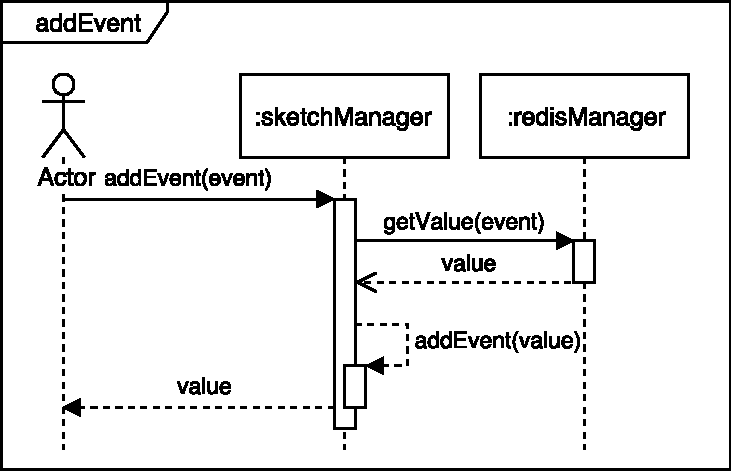
\includegraphics[width=0.45\textwidth]{../informe_2/graph/SecDiag-resourceAddEvent.pdf}
	\caption{Diagrama de secuencia para nuevos eventos (segundo incremento)}
	\label{fig:SecDiagResourceAddEvent}
\end{figure}

En lugar de ser enviados directamente por un actor, el componente está suscripto a un canal particular de la cola de mensajes, escuchando nuevos eventos publicados en el mismo. Mediante un \textit{callback}, cada vez que un evento nuevo es publicado, el componente es notificado y obtiene el mensaje del canal. Aquí, podemos clasificar el mecanismo de lectura de mensajes como \textit{push}, es decir, un actor empuja eventos al servicio, y \textit{pull}, donde el servicio lee u obtiene los eventos de un origen de datos dado (en este caso, una cola de mensajes).

\newpage
\nocite{*}
\printbibliography

\end{document}

